%% ใช้ XeLaTeX Compiler (ใน Overleaf เลือกที่ Menu)
% !TEX program = xelatex
\documentclass[11pt,a4paper]{article}

%% ---- LaTeX syntax utility package ---- %%
\usepackage{etoolbox}

%% ---- Set up paper margin ---- %%
\usepackage[a4paper,top=1in,bottom=1.25in,left=1.25in,right=1in]{geometry}

%% ---- Set up fonts and encoding ---- %%
\usepackage{fontspec}
\usepackage{xunicode}
\usepackage{xltxtra}
\usepackage{gensymb}
\usepackage{comment}


% Enable line breaks for Thai text
\XeTeXlinebreaklocale "th"
\XeTeXlinebreakskip = 0pt plus 2pt minus 1pt

% Set up Thai/Eng fonts
\newfontfamily{\thaifont}{Laksaman}[Scale=MatchLowercase]
\newfontfamily{\englishfont}{CMU Serif}[Scale=MatchLowercase]
\setmainfont{CMU Serif}
%
\usepackage[Latin, Thai]{ucharclasses}
\setTransitionTo{Thai}{\thaifont}
\setTransitionFrom{Thai}{\englishfont}

%% ---- Load line spacing package ---- %%
\usepackage{setspace}

% Introducing hair space 
\newrobustcmd{\hrsp}{\ifmmode\mskip1mu\else\kern0.0625em\fi}

%% ---- Set up hyperlinks and colors ---- %%
\usepackage{xcolor}
\usepackage[unicode=true]{hyperref}
\hypersetup{%
    colorlinks,%
    linkcolor={red!50!black},%
    citecolor={blue!50!black},%
    urlcolor={blue!80!black},%
}
\renewcommand\UrlFont{\normalfont}
%
\usepackage{physics} % สำหรับพิมพ์เครื่องหมายและสัญลักษณ์ในฟิสิกส์
\usepackage{booktabs}
\usepackage{siunitx} % สำหรับพิมพ์ปริมาณในหน่วย SI
\usepackage{lipsum}
\usepackage{amsmath}
\sisetup{unit-mode = text}% ทำให้พิมพ์สัญลักษณ์ micro และ degree ได้ถูกต้อง
%
\usepackage{tikz} % สำหรับวาด diagram
\usepackage{titling}
%
\newcommand{\subtitle}[1]{%
  \posttitle{%
    \par\end{center}
    \begin{center}\large#1\end{center}
    \vskip0.5em}%
}
\usepackage{multirow} %สำหรับ merge rows

%% ------- Document starts here ------- %%
\begin{document}
%เปลี่ยนเป็นศัพท์ภาษาไทย
\renewcommand{\tablename}{ตารางที่}
\renewcommand{\figurename}{รูปที่}


\title{Laboratory Report of Physics \\ 
	\textbf{Lab: Magnetic force probe}
}
\subtitle{SCPY294 Intermediate Physics Laboratory \\ Department of Physics, Faculty of Science, Mahidol University}
\author{
\textbf{Kritin Wiwatyothin}\\
\\
Teaching Assistant: Withheld for privacy
}

\date{
Experiment conducted: January 2026\\
Report submitted: February 2026
}

\maketitle
\hrule


%% --------------------------------------- %%

\section{บทนำ} \label{introduction}
การทดลองนี้เป็นการศึกษาการสั่นของระบบคานบาง (reed) และการประยุกต์ใช้เป็น Magnetic Force Probe 
โดยอาศัยหลักการที่ว่าเมื่อมีแรงแม่เหล็กไม่สม่ำเสมอมากระทำที่ปลายคานบางขณะสั่น 
ความถี่กำทอน (resonance frequency) ของระบบจะเปลี่ยนแปลงไป 
ข้อมูลที่ได้จะนำมาวิเคราะห์เพื่อหาความสัมพันธ์ระหว่างความถี่กำทอนกับแรงแม่เหล็กภายนอก 
และนำไปใช้ค้นหาตำแหน่งและความลึกของแม่เหล็กที่ซ่อนอยู่ในกล่องดำ \cite{labmanual}

\subsection*{วัตถุประสงค์} \label{objective}
\begin{enumerate}
    \item เพื่อศึกษาการเกิดกำทอนของระบบคานบางที่ถูกทำให้สั่น
    \item เพื่อศึกษาการเปลี่ยนแปลงของความถี่กำทอนของระบบเมื่อมีแรงไม่สม่ำเสมอภายนอกมากระทำ
    \item เพื่อประยุกต์ใช้ระบบคานบางที่ถูกทำให้สั่นเป็น magnetic force probe 
    สำหรับค้นหาตำแหน่งของแม่เหล็กในกล่องดำ
\end{enumerate}

\subsection*{ทฤษฎี} \label{theory}

การสั่นกำทอน (Resonance) คือปรากฏการณ์ที่ระบบสั่นด้วยแอมพลิจูดสูงสุด 
เมื่อได้รับแรงขับที่มีความถี่ตรงกับความถี่ธรรมชาติของระบบ 
สำหรับคานบาง (reed) ที่มีปลายด้านหนึ่งยึดติดกับที่ และปลายอีกด้านสั่นอย่างอิสระ 
ความคมชัดของการสั่นกำทอนแสดงด้วย quality factor $Q$ ดังสมการ \cite{halliday,serway}
\begin{equation}
    Q = \frac{f_r}{\Delta f} \label{eq:Q_factor}
\end{equation} 
โดยที่ $f_r$ คือความถี่กำทอน และ $\Delta f = f_2 - f_1$ คือช่วงความถี่ที่สัมพันธ์กับค่ากำลังครึ่งหนึ่งของค่าสูงสุด
จากกราฟ $P_{av}$ กับ $f$

เมื่อมีแรงแม่เหล็กไม่สม่ำเสมอ (non-uniform magnetic force) มากระทำที่ปลายคานบาง 
ความถี่กำทอนจะเปลี่ยนแปลงไปจากค่าเดิม $f_{r0}$ โดยกำหนดให้
\begin{equation}
    \Delta f_r = f_r - f_{r0} \label{eq:delta_fr}
\end{equation}
ซึ่งการเปลี่ยนแปลงดังกล่าวขึ้นอยู่กับขนาดของแรงแม่เหล็กที่กระทำ 
และมีความสัมพันธ์กับระยะห่างระหว่าง tip magnet ($M_T$) กับ target magnet

ในการทดลองนี้ แอมพลิจูด $A$ ของการสั่นจะถูกวัดจากการสะท้อนของแสงเลเซอร์บนฉาก 
ขณะที่ปรับความถี่ของสัญญาณขับ (driving signal) จาก sine wave generator 
จากนั้นนำข้อมูลมาสร้างกราฟเพื่อหาค่า $f_{r0}$ และ $Q$ ของระบบ

\bigskip
\noindent
\bigskip
\noindent
\textbf{ความสัมพันธ์ระหว่างความถี่กำทอนและระยะห่างระหว่างแท่งแม่เหล็ก} \\

ในการทดลองนี้ แรงแม่เหล็กที่กระทำต่อ tip magnet ($M_T$) ที่ปลายคานบางมาจาก
calibrating magnet ($M_C$) ซึ่งถูกติดตั้งให้เคลื่อนที่ได้ในแนวดิ่ง
เมื่อระยะห่างในแนวดิ่งระหว่างแท่งแม่เหล็กทั้งสองเปลี่ยนแปลง
แรงแม่เหล็กและความถี่กำทอนจะเปลี่ยนแปลงตามไปด้วย
โดยสามารถสมมติให้ความถี่กำทอน $f_r$ เป็นฟังก์ชันของระยะห่าง $d$ ในรูปแบบดังนี้ \cite{labmanual}
\begin{equation}
    f_r(d) = A e^{-\alpha d} + f_{r0} \label{eq:fr_model}
\end{equation}
โดยที่ $A$ และ $\alpha$ เป็นค่าคงที่ และ $f_{r0}$ คือความถี่กำทอนของระบบเมื่อไม่มีแรงแม่เหล็กภายนอกมากระทำ
(กล่าวคือเมื่อ $d \to \infty$ จะได้ $f_r \to f_{r0}$)

จากนิยามของ $\Delta f_r$ ในสมการ~\eqref{eq:delta_fr} และสมการ~\eqref{eq:fr_model} จะได้
\begin{equation}
    \Delta f_r = f_r(d) - f_{r0} = A e^{-\alpha d} \label{eq:deltafr_exp}
\end{equation}
เมื่อนำ logarithm ธรรมชาติทั้งสองข้างของสมการ~\eqref{eq:deltafr_exp} จะได้ \cite{labmanual}
\begin{equation}
    \ln(\Delta f_r) = \ln(A) - \alpha d \label{eq:calib}
\end{equation}
สมการ~\eqref{eq:calib} แสดงให้เห็นว่าความสัมพันธ์ระหว่าง $\ln(\Delta f_r)$ กับ $d$ เป็นเส้นตรง
โดยมีความชัน $-\alpha$ และจุดตัดแกน $y$ เท่ากับ $\ln(A)$
กราฟดังกล่าวจึงถูกใช้เป็น calibrating graph สำหรับการหาความลึกของแท่งแม่เหล็กในกล่องดำ
กล่าวคือเมื่อทราบค่า $\ln(\Delta f_r)$ ที่วัดได้จากการทดลอง
ก็สามารถหาค่าระยะห่าง $d$ ได้จากกราฟนี้โดยตรง





%% --------------------------------------- %%
\section{ขั้นตอนการทดลอง} \label{procedure}

\subsection*{ตอนที่ 1 (การทดลอง I-A): การวัดความถี่กำทอน}
ในส่วนนี้มีวัตถุประสงค์เพื่อหาความถี่กำทอน $f_{r0}$ และ quality factor $Q$ 
ของระบบคานบางเมื่อไม่มีแรงแม่เหล็กภายนอกมากระทำ โดยมีขั้นตอนดังนี้:
\begin{enumerate}
    \item จัดชุดทดลองตามแผนภาพในรูปที่ \ref{fig:setup_A} โดยต่อแหล่งกำเนิดความต่างศักย์ 
    5V-DC เข้ากับกล่องเลเซอร์ และต่อสัญญาณขับ sine wave จาก sine wave generator 
    เข้ากับกล่องที่มีคานบาง
    \item ปรับค่า output voltage ของ sine wave generator ให้เหมาะสม
    \item จัดให้ลำแสงเลเซอร์ตกกระทบบนกระจกที่ปลายคานบาง 
    และสะท้อนมาตกบนฉากเพื่อใช้วัดแอมพลิจูด $A$ ของการสั่น
    \item ปรับความถี่ของสัญญาณขับ $f$ ในช่วงที่เหมาะสมรอบค่าความถี่กำทอน 
    และบันทึกค่าแอมพลิจูด $A$ ที่แต่ละความถี่
    \item วาดกราฟความสัมพันธ์ระหว่าง $A^2$ กับ $f$ 
    และหาค่าความถี่กำทอน $f_{r0}$ จากตำแหน่งที่แอมพลิจูดมีค่าสูงสุด
    \item คำนวณค่า quality factor จากสมการ~\eqref{eq:Q_factor} 
    โดยใช้ค่า $\Delta f = f_2 - f_1$ ที่อ่านได้จากกราฟ 
    ณ ตำแหน่งที่กำลังมีค่าเท่ากับครึ่งหนึ่งของกำลังสูงสุด หรือที่ตำแหน่ง $y = \frac{A^2_{max}}{2}$
\end{enumerate}

\subsection*{ตอนที่ 2 (การทดลอง I-B): ความสัมพันธ์ระหว่างความถี่กำทอนและแรงภายนอก}
ในส่วนนี้มีวัตถุประสงค์เพื่อศึกษาการเปลี่ยนแปลงของความถี่กำทอนเมื่อมีแรงแม่เหล็ก
ไม่สม่ำเสมอมากระทำ และสร้าง calibrating graph สำหรับใช้ในตอนที่ 3 
โดยมีขั้นตอนดังนี้:
\begin{enumerate}
    \item ติดตั้ง calibrating magnet $M_C$ บน slider โดยให้ขั้วเหนืออยู่ด้านบน 
    และจัดให้ tip magnet $M_T$ กับ $M_C$ อยู่บนแนวเส้นดิ่งเดียวกัน
    \item ปรับระยะห่างในแนวดิ่ง $d$ ระหว่าง $M_T$ และ $M_C$ 
    ตั้งแต่ระยะห่างมากจนถึงระยะห่างน้อยที่สุดที่ทำได้ 
    และบันทึกค่าความถี่กำทอน $f_r$ ที่แต่ละค่า $d$
    \item วาดกราฟความสัมพันธ์ระหว่าง $f_r$ กับ $d$
    \item คำนวณ $\Delta f_r = f_r - f_{r0}$ 
    และวาดกราฟระหว่าง $\ln(\Delta f_r)$ กับ $d$ 
    ซึ่งควรได้กราฟเส้นตรงตามสมการ~\eqref{eq:calib} 
    กราฟนี้จะถูกใช้เป็น calibrating graph ในตอนที่ 3
\end{enumerate}

\subsection*{ตอนที่ 3 (การทดลอง I-C): การหาตำแหน่งและความลึกของแท่งแม่เหล็กในกล่องดำ}
ในส่วนนี้มีวัตถุประสงค์เพื่อประยุกต์ใช้ magnetic force probe 
ค้นหาตำแหน่งและความลึกของแท่งแม่เหล็ก $M_A$ และ $M_B$ 
ที่ซ่อนอยู่ในกล่องดำ โดยมีขั้นตอนดังนี้:
\begin{enumerate}
    \item สำหรับแท่งแม่เหล็ก $M_A$ ซึ่งทราบตำแหน่งในแนวระดับแล้วจากเส้นปะที่กำหนดให้บนกล่องดำ
    นำ tip magnet $M_T$ ไปวางเหนือตำแหน่งดังกล่าว 
    และวัดค่าความถี่กำทอน $f_r$ ที่ได้ 
    จากนั้นคำนวณ $\Delta f_r = f_r - f_{r0}$ 
    แล้วนำค่าที่ได้ไปเทียบกับ calibrating graph จากตอนที่ 2 
    เพื่อหาความลึก $d_A$ ของ $M_A$ จากผิวกล่องดำด้านบน
    \item สำหรับแท่งแม่เหล็ก $M_B$ ซึ่งทราบเพียงตำแหน่งในแนวแกน $y$ 
    ให้เลื่อน $M_T$ สแกนไปตามแนวแกน $x$ บนผิวกล่องดำที่ค่า $y$ ดังกล่าว โดยปรับความถี่ของสัญญาณเป็นค่าหนึ่ง (แนะนำให้เป็นความถี่ที่ทำให้เกิด $A$ สูงสุดจากตอนที่ 1 เพื่อให้สังเกตพฤติกรรมได้ง่าย) จากนั้นบันทึกค่าความถี่กำทอน $f_r$ ณ แต่ละตำแหน่ง $x$
    \item วาดกราฟความสัมพันธ์ระหว่าง $f_r$ กับตำแหน่ง $x$ 
    กราฟที่ได้ควรมีลักษณะเป็นรูปภูเขา โดยมีค่าสูงสุดคือที่ตำแหน่งของ $M_B$ ในแนวระดับ
\end{enumerate}

\begin{figure}[htbp]
    \centering
    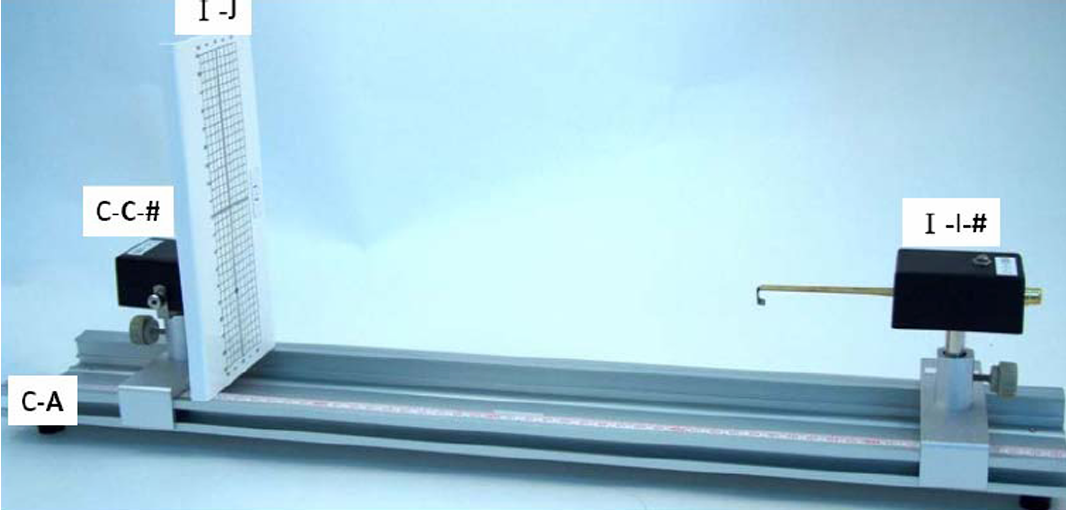
\includegraphics[width=0.8\textwidth]{setup_IA.png}
    \caption{ชุดทดลองสำหรับการวัดความถี่กำทอนในการสั่นของคานบาง (การทดลอง I-A)}
    \label{fig:setup_A}
\end{figure}

\begin{figure}[htbp]
    \centering
    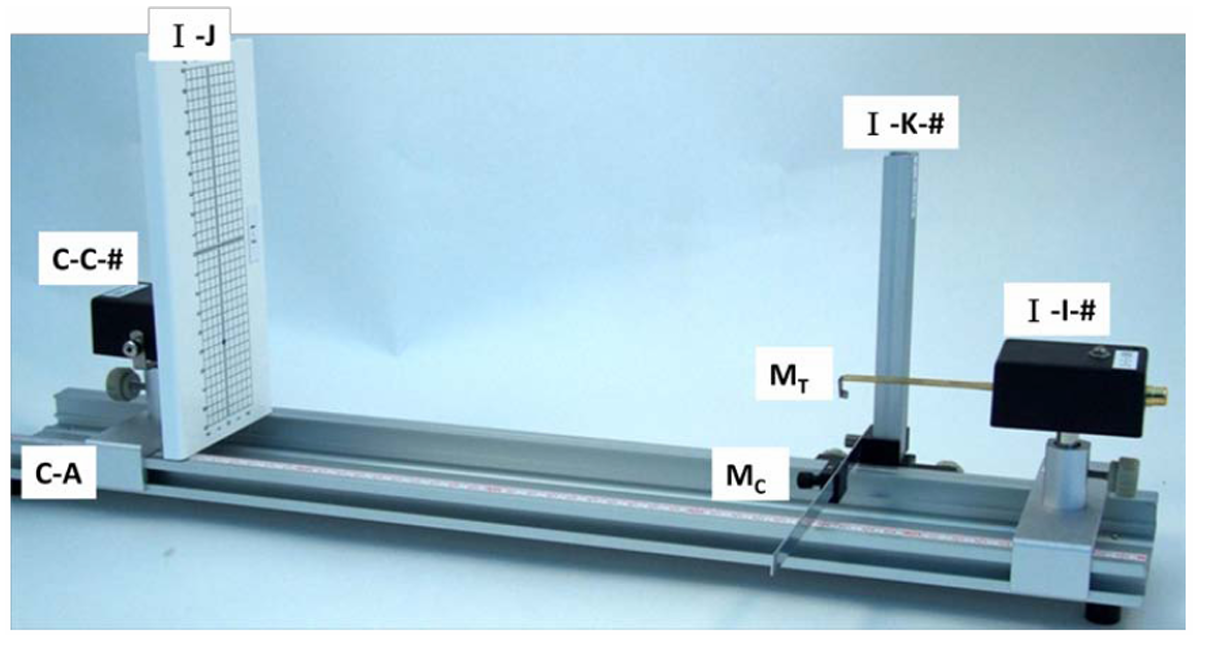
\includegraphics[width=0.8\textwidth]{setup_IB.png}
    \caption{ชุดทดลองสำหรับการทดลอง I-B 
    แสดง calibrating magnet $M_C$ และ tip magnet $M_T$}
    \label{fig:setup_B}
\end{figure}




%% --------------------------------------- %%
\newpage
\section{ผลการทดลอง} \label{result}

\subsection{ข้อมูลจากการทดลอง} \label{data}
จากการทดลองเพื่อศึกษา Magnetic force probe กำหนดให้การวัดความถี่มีค่าความคลาดเคลื่อนเครื่องมือ $\pm 0.01$ Hz  และการอ่านค่าจากสเกลบนฉากมีค่าความคลาดเคลื่อน $\pm 0.1$ cm  นอกจากนี้การทดลองตอนที่ 3 ได้มีการตั้งค่าความถี่ไว้ที่ $26.50 \pm 0.01$ Hz โดยในการทดลองนี้ไม่ต้องคำนวณ Error จากการวัดตามคำแนะนำในคู่มือปฏิบัติการ ทำให้ได้ตารางข้อมูลดังนี้

\begin{table}[htbp]
\centering
\caption{ความสัมพันธ์ระหว่างความถี่ ($f$) และแอมพลิจูด ($A$) ของการสั่นของคานบาง}
\renewcommand{\arraystretch}{1.2}
\begin{tabular}{|c|c|c|}
\hline
ความถี่ $f$ ($\pm 0.01$ Hz) & ค่าที่อ่านจากสเกล ($\pm 0.1$ cm) & แอมพลิจูด $A$ ($\pm 0.1$ cm) \\
\hline
0 & -0.6 & 0.0 \\
26.03 & 0.7 & 1.3 \\
26.08 & 1.0 & 1.6 \\
26.12 & 1.1 & 1.7 \\
26.13 & 1.2 & 1.8 \\
26.14 & 1.2 & 1.8 \\
26.16 & 1.3 & 1.9 \\
26.18 & 1.3 & 1.9 \\
26.20 & 1.4 & 2.0 \\
26.22 & 1.3 & 1.9 \\
26.24 & 1.2 & 1.8 \\
26.26 & 1.2 & 1.8 \\
26.28 & 1.1 & 1.7 \\
26.30 & 1.1 & 1.7 \\
26.32 & 1.0 & 1.6 \\
26.34 & 0.9 & 1.5 \\
26.36 & 0.9 & 1.5 \\
26.38 & 0.8 & 1.4 \\
26.40 & 0.7 & 1.3 \\
\hline
\end{tabular}
\end{table}

\begin{table}[htbp]
\centering
\caption{ความสัมพันธ์ระหว่างความถี่กำทอน ($f_r$) และระยะห่างในแนวดิ่ง ($d$)}
\renewcommand{\arraystretch}{1.2}
\begin{tabular}{|c|c|}
\hline
ระยะห่าง $d$ ($\pm 0.1$ cm) & ความถี่กำทอน $f_r$ (Hz) \\
\hline
5.3 & 27.20 $\pm$ 0.03 \\
5.2 & 26.89 $\pm$ 0.02 \\
5.1 & 26.80 $\pm$ 0.04 \\
5.0 & 26.65 $\pm$ 0.05 \\
4.9 & 26.51 $\pm$ 0.03 \\
4.8 & 26.44 $\pm$ 0.05 \\
4.7 & 26.40 $\pm$ 0.04 \\
4.6 & 26.33 $\pm$ 0.03 \\
4.5 & 26.31 $\pm$ 0.04 \\
4.4 & 26.28 $\pm$ 0.03 \\
4.3 & 26.28 $\pm$ 0.03 \\
\hline
\end{tabular}
\end{table}
\textbf{\underline{หมายเหตุ}} $d$ ในที่นี้คือ **ค่าตำแหน่งที่อ่านได้จากไม้บรรทัด** โดย ณ ตำแหน่งที่ $d=5.3$ cm คือตำแหน่งที่ใกล้แม่เหล็ก $M_T$ ที่สุด และลดลงเรื่อยๆตามลำดับ

\begin{table}[htbp]
\centering
\caption{การหาตำแหน่งแม่เหล็ก $M_B$ ในแนวระดับ ($x$)}
\renewcommand{\arraystretch}{1.2}
\begin{tabular}{|c|c|c|}
\hline
ตำแหน่งสเกล ($\pm 0.1$ cm) & $x$ ($\pm 0.1$ cm) & $A$ ($\pm 0.1$ cm) \\
\hline
5.9 (ขอบกล่อง) & 0.0 & 2.9 \\
6.1 & 0.2 & 3.0 \\
6.3 & 0.4 & 3.1 \\
6.5 & 0.6 & 3.2 \\
6.7 & 0.8 & 3.3 \\
6.8 & 0.9 & 3.4 \\
7.0 & 1.1 & 3.3 \\
7.2 & 1.3 & 3.2 \\
7.4 & 1.5 & 3.0 \\
\hline
\end{tabular}
\end{table}

ในส่วนของตำแหน่งแม่เหล็ก $M_A$ จะมีความถี่ $f_r$ ในช่วง $26.46 \pm 0.03$ Hz


\newpage
\newpage
\subsection{การคำนวณความคลาดเคลื่อน}

ค่าความคลาดเคลื่อนที่เกิดขึ้นในการทดลองนี้มีแหล่งที่มาหลักจากการอ่านตำแหน่งบนสเกลของฉากรับแสงเพื่อหาแอมพลิจูด, ความไม่แน่นอนในการระบุความถี่กำทอนจากการวัด และความคลาดเคลื่อนสะสมจากการใช้แบบจำลองทางคณิตศาสตร์ (Calibration model) เพื่อหาความลึกของแม่เหล็ก โดยสามารถแบ่งแหล่งที่มาได้ดังนี้

\subsubsection{ความคลาดเคลื่อนของแอมพลิจูด $A$}

ในการวัดแอมพลิจูดของการสั่น ($A$) แอมพลิจูดเกิดจากระยะห่างระหว่างตำแหน่งสูงสุดที่อ่านได้บนฉาก ($y_{max}$) ลบกับตำแหน่งสมดุลขณะหยุดนิ่ง ($y_0$) โดยไม้บรรทัดที่ติดบนฉากมีความละเอียดต่ำสุดเท่ากับ $0.1$ cm จึงกำหนดให้ความคลาดเคลื่อนจากการอ่านตำแหน่งแต่ละครั้งเป็น $\sigma_{y} = 0.1$ cm 

เนื่องจากแอมพลิจูดคำนวณจาก $A = y_{max} - y_0$ ความคลาดเคลื่อนเชิงระบบของแอมพลิจูด ($\sigma_{A}$) จึงคำนวณได้จาก Gaussian error propagation ดังนี้
\[
\sigma_{A} = \sqrt{\sigma_{y_{max}}^2 + \sigma_{y_0}^2} = \sqrt{2\sigma_{y}^2} = \sqrt{2}(0.1) \approx 0.14 \text{ cm}
\]
ทั้งนี้ ตามข้อกำหนดที่ให้พิจารณาความคลาดเคลื่อนที่มีนัยสำคัญเพียง 1 ตำแหน่ง จะได้ว่า $\sigma_A \approx 0.1$ cm ในการรายงานผลในตารางถัดไป

\subsubsection{ความคลาดเคลื่อนของความถี่กำทอน $f_r$ และ $\Delta f_r$}

ความคลาดเคลื่อนของความถี่ขับ ($f$) มาจากความละเอียดของเครื่องกำเนิดสัญญาณ (Sine wave generator) ซึ่งอ่านค่าได้ละเอียดถึง $0.01$ Hz ($\sigma_f = 0.01$ Hz) 

สำหรับการเปลี่ยนแปลงของความถี่กำทอน $\Delta f_r = f_r - f_{r0}$ ซึ่งเป็นการลบกันของค่าความถี่สองค่า ความคลาดเคลื่อนจึงเป็น
\[
\delta \Delta f_r = \sqrt{(\sigma_{f_r})^2 + (\sigma_{f_{r0}})^2}
\]
โดยที่ $\sigma_{f_r}$ และ $\sigma_{f_{r0}}$ คือความไม่แน่นอนในการตัดสินใจเลือกจุดที่เกิดแอมพลิจูดสูงสุดในแต่ละสภาวะ

\subsubsection{ความคลาดเคลื่อนของระยะห่างระหว่างแม่เหล็ก $d$}

ในขั้นตอนการทำ Calibration (ตอนที่ 2) ระยะห่าง $d$ วัดจากสเกลบนรางเลื่อนที่มีความละเอียด $0.1$ cm ดังนั้น $\sigma_d = 0.1$ cm 

อย่างไรก็ตาม ในขั้นตอนการหาความลึกของแม่เหล็ก $M_A$ ในกล่องดำ (ตอนที่ 3) ค่า $d$ จะได้มาจากการแก้สมการ Model $f_r(d) = A e^{-\alpha d} + f_{r0}$ ดังนั้นความคลาดเคลื่อนของ $d$ จะขึ้นอยู่กับทั้งความคลาดเคลื่อนของพารามิเตอร์จากการ Fit ($A, \alpha, f_{r0}$) และความคลาดเคลื่อนของความถี่ $f_r$ ที่วัดได้จริงหน้างาน
\[
\sigma_{d} = \sqrt{ \left( \abs{\frac{\partial d}{\partial f_r}} \delta f_r \right)^2 + \sum \left( \abs{\frac{\partial d}{\partial p_i}} \delta p_i \right)^2 }
\]
โดยที่ $p_i$ คือพารามิเตอร์ $A$ และ $\alpha$ ที่ได้จากกระบวนการ Least squares regression

\subsubsection{ความคลาดเคลื่อนของ Quality Factor $Q$}

ค่า Quality Factor คำนวณจาก $Q = f_r / (f_2 - f_1)$ ความคลาดเคลื่อนสัมพัทธ์คำนวณได้ดังนี้
\[
\frac{\delta Q}{Q} = \sqrt{ \left( \frac{\delta f_r}{f_r} \right)^2 + \left( \frac{\sqrt{\delta f_2^2 + \delta f_1^2}}{f_2 - f_1} \right)^2 }
\]







%% -------------------------------------------- %%

\newpage
\section{การวิเคราะห์ผลและอภิปรายผล} \label{analysis}

\subsection{การหาค่าความถี่กำทอนและ Quality Factor (ตอนที่ 1)}

จากข้อมูลความสัมพันธ์ระหว่างความถี่ขับ ($f$) และแอมพลิจูด ($A$) ในตารางที่ 1 เมื่อนำมาวิเคราะห์หาค่ากำลังเฉลี่ย ($P_{av} \propto A^2$) พบพฤติกรรมการตอบสนองแบบกำทอนที่ชัดเจน โดยมีรายละเอียดดังนี้

\begin{figure}[htbp]
    \centering
    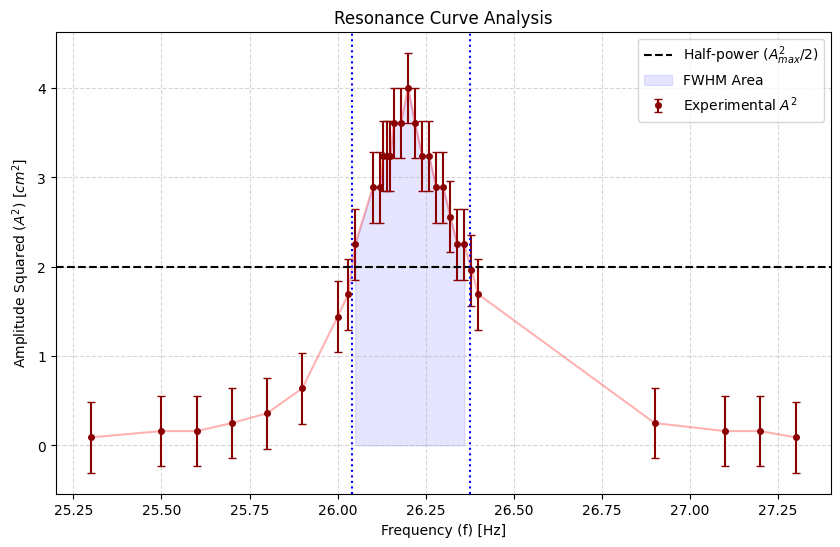
\includegraphics[width=1\textwidth]{ResonanceCurve.png} 
    \caption{กราฟแสดงความสัมพันธ์ระหว่าง $A^2$ กับความถี่ $f$}
    \label{fig:part1}
\end{figure}

\begin{itemize}
    \item ความถี่กำทอนธรรมชาติ: $f_{r0} = 26.20 \pm 0.01$ Hz
    \item ช่วงความถี่ที่กำลังครึ่งหนึ่ง ($\Delta f = f_2 - f_1$): $0.34$ Hz
    \item ค่า Quality Factor ($Q$) ที่คำนวณได้: $Q = 78 \pm 7$
\end{itemize}
ค่า $Q$ ที่สูง (ประมาณ 78) แสดงให้เห็นว่าระบบคานบางมีการสูญเสียพลังงานต่ำ (Low damping) และมีการตอบสนองต่อความถี่ที่แหลมคม (Sharp resonance) ซึ่งเป็นคุณสมบัติที่เหมาะสมในการนำมาใช้เป็นหัววัด (Probe) เนื่องจากแรงภายนอกเพียงเล็กน้อยจะส่งผลต่อการเปลี่ยนแปลงพฤติกรรมการสั่นได้อย่างชัดเจน

\subsection{ความสัมพันธ์ระหว่างความถี่กำทอนและระยะห่าง (ตอนที่ 2)}

ในการสร้างกราฟมาตรฐาน (Calibration) ได้ขยับแม่เหล็ก $M_C$ เข้าหาปลายคาน โดย $d$ ในที่นี้คือ **ค่าตำแหน่งที่อ่านได้จากไม้บรรทัด** ซึ่งจากข้อมูลพบว่าตำแหน่ง $d = 5.3$ cm เป็นจุดที่ใกล้แม่เหล็กมากที่สุด และ $d = 4.3$ cm เป็นจุดที่ไกลที่สุด เมื่อพิจารณาความสัมพันธ์ระหว่างความถี่กำทอน ($f_r$) กับตำแหน่ง $d$ พบว่ายิ่งเข้าใกล้แม่เหล็ก ความถี่จะยิ่งสูงขึ้นตามแบบจำลอง $f_r(d) = A e^{\alpha d} + f_{r0}$ (โดย $\alpha$ มีค่าเป็นบวกเพื่อแสดงการเพิ่มขึ้นตามค่า $d$)

\begin{figure}[htbp]
    \centering
    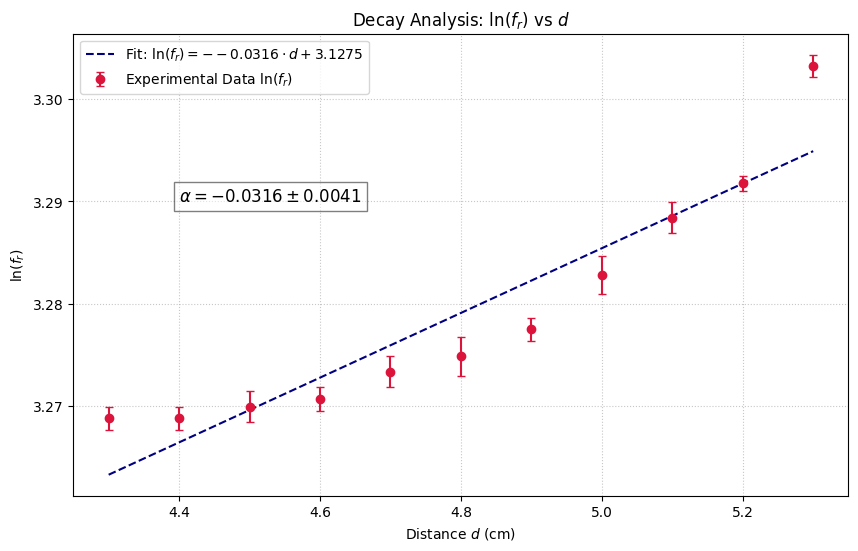
\includegraphics[width=1\textwidth]{Calibration_Graph.png} 
    \caption{กราฟแสดงความสัมพันธ์ระหว่าง $\ln(\Delta f_r)$ กับระยะห่าง $d$ (Calibration Curve)}
    \label{fig:calib_graph}
\end{figure}

\begin{itemize}
    \item สัมประสิทธิ์การลดทอน ($\alpha$): $0.032 \pm 0.004 \text{ cm}^{-1}$
    \item ค่าคงที่จากการฟิต ($\ln A$): $3.13$
\end{itemize}

\subsection{การระบุตำแหน่งและความลึกของแม่เหล็กในกล่องดำ (ตอนที่ 3)}

\subsubsection{การวิเคราะห์แม่เหล็ก $M_A$}
จากการวัดความถี่กำทอนเหนือตำแหน่งแม่เหล็ก $M_A$ ได้ค่า $f_r = 26.46 \pm 0.03$ Hz เมื่อนำมาคำนวณหาความลึกผ่านแบบจำลองการถดถอย (Regression model) โดยใช้หลักการส่งผ่านความคลาดเคลื่อน (Error propagation) พบว่า:
\begin{quote}
    \textbf{ความลึกของแม่เหล็ก $M_A$ จากผิวกล่อง ($d_A$):} $4.84 \pm 0.05$ cm
\end{quote}

\subsubsection*{การวิเคราะห์ตำแหน่งแม่เหล็ก $M_B$ ด้วยแบบจำลองเกาส์เซียน (Gaussian Fit)}

ในการระบุตำแหน่งศูนย์กลางของแม่เหล็ก $M_B$ ในแนวระดับอย่างแม่นยำ แทนที่จะใช้การลากเส้นเชื่อมต่อระหว่างจุดข้อมูลซึ่งอาจมีความคลาดเคลื่อนจากการอ่านสเกลในแต่ละครั้ง หรือการวาดแนวโน้มด้วยมือ การทดลองนี้เลือกใช้การฟิตข้อมูลด้วยแบบจำลองการกระจายตัวแบบเกาส์เซียน (Gaussian Distribution) ตามสมการ:
\begin{equation}
    A(x) = a \cdot e^{-\frac{(x-\mu)^2}{2\sigma^2}} + c
\end{equation}
โดยที่ $\mu$ คือตำแหน่งศูนย์กลางของแม่เหล็กที่ทำให้เกิดแอมพลิจูดสูงสุด เหตุผลที่เลือกใช้โมเดลนี้เนื่องจากอันตรกิริยาของสนามแม่เหล็กในแนวราบระหว่าง $M_T$ และ $M_B$ มีลักษณะลดหลั่นลงอย่างสมมาตรรอบจุดศูนย์กลาง ซึ่งสอดคล้องกับพฤติกรรมรูปทรงระฆังคว่ำ (Bell-shaped curve)

\begin{figure}[htbp]
    \centering
    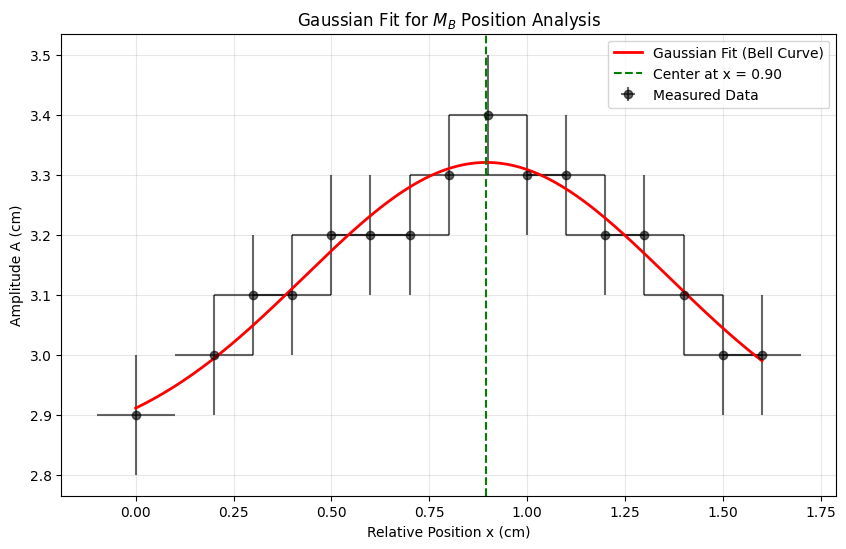
\includegraphics[width=1\textwidth]{Part3Graph.png}
    \caption{กราฟแสดงการฟิตข้อมูลแอมพลิจูด $A$ และตำแหน่ง $x$ ด้วย Gaussian Function}
    \label{fig:gaussian_mb}
\end{figure}

จากผลการคำนวณด้วยวิธี Least squares พบว่าพารามิเตอร์ $\mu$ ซึ่งระบุตำแหน่งศูนย์กลางมีค่าเท่ากับ $0.896 \pm 0.022$ cm เพื่อให้สอดคล้องกับเงื่อนไขการรายงานผลที่มีนัยสำคัญ 1 ตำแหน่ง จึงสรุปได้ว่า:
\begin{quote}
    \textbf{ตำแหน่งของแม่เหล็ก $M_B$ ในแนวระดับ:} $x = 0.9 \pm 0.1$ cm
\end{quote}
ถึงแม้ว่าพฤติกรรมระหว่าง $x$ และ $A$ จะไม่ได้มีฟังก์ชันที่แน่นอน แต่ผู้ทดลองคิดว่าการใช้ฟังก์ชันที่มีหน้าตาสอดคล้องกับผลการทดลองมาฟิต จะให้ผลลัพธ์ที่น่าเชื่อถือ และมีหลักการมากกว่าการลากประมาณด้วยมือ เพราะอย่างน้อยการฟิตแบบนี้เท่าให้เราสามารถย้อนหรือประมาณจุดข้อมูลได้คร่าวๆ

\subsection{วิจารณ์ผลการทดลอง}
ความคลาดเคลื่อนของ $d_A$ ($\pm 0.05$ cm) มีค่าน้อยกว่าความคลาดเคลื่อนจากการอ่านสเกลโดยตรง ($\pm 0.1$ cm) ส่วนหนึ่งเป็นผลมาจากการใช้กระบวนการฟิตข้อมูลเชิงสถิติที่ช่วยลดความไม่แน่นอน อย่างไรก็ตามระบบคานบางที่มีค่า $Q$ สูง ยังคงช่วยให้แยกแยะความแตกต่างของความถี่ได้ในระดับ $0.01$ Hz ทำให้ Magnetic Force Probe นี้มีประสิทธิภาพเพียงพอในการตรวจวัดวัตถุที่ซ่อนอยู่


\newpage
\section*{อภิปรายผล}

จากการทดลองนี้ ได้ทำการศึกษาพฤติกรรมการสั่นของระบบคานบาง และการประยุกต์ใช้เป็นหัววัดแรงแม่เหล็ก โดยอาศัยการเปลี่ยนแปลงของความถี่กำทอนเมื่อมีแรงแม่เหล็กภายนอกมากระทำ ซึ่งผลการทดลองสามารถอภิปรายได้ตามประเด็นสำคัญดังนี้

\textbf{ในส่วนของคุณลักษณะของหัววัด (ตอนที่ 1)} พบว่าระบบคานบางมีพฤติกรรมการตอบสนองแบบกำทอนที่ชัดเจนมาก โดยมีค่า Quality Factor ($Q$) สูงถึง $78 \pm 7$ ค่า $Q$ ที่สูงนี้สะท้อนถึงการสูญเสียพลังงานในระบบที่ต่ำ (Low damping) ทำให้กราฟการสั่นมีความคมชัด ซึ่งเป็นหัวใจสำคัญของการทำเป็น Probe เนื่องจากแรงแม่เหล็กเพียงเล็กน้อยจะส่งผลให้ตำแหน่งของความถี่กำทอนขยับไปได้อย่างมีนัยสำคัญ ทำให้เราสามารถตรวจวัดการเปลี่ยนแปลงได้แม่นยำ

\textbf{ในส่วนของการสร้างกราฟมาตรฐาน (ตอนที่ 2)} เมื่อนำแม่เหล็ก $M_C$ เข้าใกล้ปลายคาน ตำแหน่งบนสเกลไม้บรรทัด $d$ ที่เพิ่มขึ้น (ซึ่งหมายถึงระยะห่างที่น้อยลง) ส่งผลให้ความถี่กำทอน $f_r$ เพิ่มขึ้นตามแบบจำลอง Exponential:
\[
f_r(d) = A e^{\alpha d} + f_{r0}
\]
จากการฟิตกราฟด้วยสมการเส้นตรง $\ln(f_r - f_{r0}) = \ln(A) + \alpha d$ ได้ค่าสัมประสิทธิ์การตอบสนอง $\alpha = 0.032 \pm 0.004 \text{ cm}^{-1}$ และ $\ln{A} \approx 3.13$

\textbf{ในการระบุตำแหน่งแม่เหล็กในกล่องดำ (ตอนที่ 3)} 
\begin{itemize}
    \item สำหรับแม่เหล็ก $M_A$ ความลึกที่คำนวณได้คือ $4.84 \pm 0.05$ cm ซึ่งสอดคล้องกับค่าคาดคะเนที่ระบุไว้ แสดงให้เห็นว่า Calibration model ที่สร้างขึ้นมีความถูกต้องและนำมาใช้งานได้จริง
    \item สำหรับแม่เหล็ก $M_B$ การใช้แบบจำลองเกาส์เซียน (Gaussian Fit) มาวิเคราะห์แอมพลิจูดในแนวระดับ ให้ค่าตำแหน่งศูนย์กลาง $\mu = 0.896 \pm 0.022$ cm หรือสรุปได้เป็น $0.9 \pm 0.1$ cm การเลือกใช้ Gaussian Fit แทนการลากเส้นด้วยมือนั้นมีข้อดีคือ ช่วยลดความคลาดเคลื่อนที่เกิดจากความไม่แน่นอนเชิงสถิติ (Random error) ของการอ่านสเกลในแต่ละจุด และให้ผลลัพธ์ที่มีหลักการทางสถิติรองรับมากกว่า
\end{itemize}

\textbf{แหล่งที่มาของความคลาดเคลื่อน} หลัก ๆ มาจากความละเอียดของอุปกรณ์วัด (ไม้บรรทัด $\pm 0.1$ cm และเครื่องกำเนิดสัญญาณ $\pm 0.01$ Hz) นอกจากนี้ยังมีปัจจัยเชิงระบบ เช่น การรบกวนจากสนามแม่เหล็กภายนอก หรือความไม่สมบูรณ์ของผิวหน้าสัมผัสของแม่เหล็ก อย่างไรก็ตาม ความคลาดเคลื่อนสุดท้ายของ $d_A$ และ $x_B$ ที่มีค่าประมาณ $0.05-0.1$ cm ถือว่าอยู่ในระดับที่ยอมรับได้สำหรับการทดลองนี้




\newpage
\section{สรุปผลการทดลอง} \label{conclusion}

การทดลองนี้ได้ศึกษาพฤติกรรมการสั่นกำทอนของระบบคานบาง และการประยุกต์ใช้เป็นหัววัดแรงแม่เหล็ก (Magnetic Force Probe) เพื่อระบุตำแหน่งและความลึกของวัตถุที่ซ่อนอยู่ โดยสามารถสรุปประเด็นสำคัญได้ดังนี้

1. ระบบคานบางที่ใช้มีคุณลักษณะการตอบสนองต่อความถี่ที่แหลมคม โดยมีค่าความถี่กำทอนธรรมชาติ $f_{r0} = 26.20 \pm 0.01$ Hz และมีค่า Quality Factor ($Q$) เท่ากับ $78 \pm 7$ ซึ่งแสดงถึงความไวสูงต่อการเปลี่ยนแปลงของแรงภายนอก

2. ความสัมพันธ์ระหว่างความถี่กำทอน ($f_r$) และตำแหน่งบนสเกลไม้บรรทัด ($d$) เป็นไปตามแบบจำลอง Exponential ซึ่งความถี่จะเพิ่มขึ้นเมื่อหัววัดเข้าใกล้แม่เหล็กมากขึ้น โดยมีสัมประสิทธิ์การตอบสนอง $\alpha = 0.032 \pm 0.004 \text{ cm}^{-1}$ และค่าคงที่จากการฟิต $\ln A = 3.13$

3. จากการนำหัววัดไปทดสอบกับกล่องดำ สามารถระบุตำแหน่งของแม่เหล็กที่ซ่อนอยู่ได้อย่างแม่นยำ ดังนี้:
\begin{itemize}
    \item \textbf{แม่เหล็ก $M_A$:} มีระดับตำแหน่งบนสเกล (ความลึก) เท่ากับ $4.84 \pm 0.05$ cm
    \item \textbf{แม่เหล็ก $M_B$:} มีตำแหน่งศูนย์กลางในแนวระดับเท่ากับ $x = 0.9 \pm 0.1$ cm (วิเคราะห์ด้วยวิธี Gaussian Fit)
\end{itemize}

ผลการทดลองแสดงให้เห็นว่าระบบคานบางที่มีค่า $Q$ สูง สามารถตรวจวัดอันตรกิริยาของแรงแม่เหล็กที่ไม่สม่ำเสมอได้อย่างมีประสิทธิภาพ โดยการวิเคราะห์ข้อมูลด้วยวิธีการฟิตฟังก์ชันทางสถิติ (Regression) ช่วยให้สามารถระบุตำแหน่งของวัตถุได้แม่นยำกว่าการสังเกตด้วยสายตาเพียงอย่างเดียว สรุปได้ว่า Magnetic Force Probe ที่สร้างขึ้นนี้สามารถทำงานได้ถูกต้องตามหลักการทางฟิสิกส์ภายในขอบเขตความคลาดเคลื่อนที่ยอมรับได้


%% --------------------------------------- %%
\newpage
\begin{thebibliography}{9}

\bibitem{labmanual}
Department of Physics, Faculty of Science, Mahidol University,
\textit{SCPY294 Intermediate Physics Laboratory Manual: Lab 05 Magnetic Force Probe},
Mahidol University, Nakhon Pathom, Thailand, 2026.

\bibitem{halliday}
David Halliday, Robert Resnick, and Jearl Walker,
\textit{Fundamentals of Physics},
11th ed.,
John Wiley \& Sons, Hoboken, NJ, 2018.

\bibitem{serway}
Raymond A. Serway and John W. Jewett, Jr.,
\textit{Physics for Scientists and Engineers with Modern Physics},
10th ed.,
Cengage Learning, Boston, MA, 2019.

\bibitem{taylor}
John R. Taylor,
\textit{An Introduction to Error Analysis: The Study of Uncertainties in Physical Measurements},
2nd ed.,
University Science Books, Sausalito, CA, 1997.

\bibitem{bevington}
Philip R. Bevington and D. Keith Robinson,
\textit{Data Reduction and Error Analysis for the Physical Sciences},
3rd ed.,
McGraw-Hill, New York, 2003.

\end{thebibliography}
%% --------------------------------------- %%
\end{document}
%